\documentclass[11pt,a4paper]{article}

% --- Packages ---
\usepackage[utf8]{inputenc}
\usepackage[T1]{fontenc}
\usepackage{amsmath,amssymb,amsfonts}
\usepackage{graphicx}
\usepackage{booktabs}
\usepackage{hyperref}
\usepackage[numbers,sort&compress]{natbib}
\usepackage[margin=1in]{geometry}
\usepackage{algorithm}
\usepackage{algorithmic}
\usepackage{multirow}
\usepackage{caption}
\usepackage{subcaption}
\usepackage{xcolor}
\usepackage{float}

% --- Hyperref setup ---
\hypersetup{
    colorlinks=true,
    linkcolor=blue,
    citecolor=blue,
    urlcolor=blue
}

% --- Custom commands ---
\newcommand{\R}{\mathbb{R}}
\newcommand{\E}{\mathbb{E}}
\newcommand{\Prob}{\mathbb{P}}

\title{Continuous Gaussian Hidden Markov Models for Equity and Volatility Index Dynamics:\\A Baum-Welch Approach Without Jump Augmentation, with Cross-Asset SIM and Copula Extensions}

\author{
    Abdulrahman Alswaidan\thanks{Cornell University, Robert Frederick Smith School of Chemical and Biomolecular Engineering, Ithaca, NY, USA. Email: \texttt{aa2725@cornell.edu}.}
    \and
    Cade Jin\thanks{Cornell University, Ithaca, NY, USA. Email: \texttt{cj383@cornell.edu}.}
    \and
    Jeffrey D.\ Varner\thanks{Cornell University, Robert Frederick Smith School of Chemical and Biomolecular Engineering, Ithaca, NY, USA. Email: \texttt{jdv27@cornell.edu}.}
}

\date{\today}

\begin{document}

\maketitle

% ========================================================================================= %
\begin{abstract}
We present a continuous hidden Markov model (CHMM) with Gaussian emissions, trained by the Baum-Welch (Expectation-Maximization) algorithm, for generating synthetic financial time series that preserve the canonical stylized facts of asset returns.
Unlike the discrete-state framework of \citet{alswaidan2026hybrid} — which requires Laplace quantile binning and a Poisson jump-duration mechanism to achieve volatility clustering — the continuous model at a single moderate state resolution ($K = 18$, chosen jointly by four information criteria \citep{nguyen2018hidden} and a seven-metric distributional score over $K \in \{3, 6, 9, 12, 15, 18, 21\}$) reproduces all three stylized facts without jump augmentation, eliminating two tunable hyperparameters and the discretization step.

On ten years of daily SPDR S\&P~500 ETF (SPY) data we benchmark the CHMM against six alternatives — bootstrap resampling, Gaussian and Laplace i.i.d., the discrete HMM of \citet{alswaidan2026hybrid} in no-jump (NJ) and Poisson-jump (WJ) variants, and GARCH(1,1) — using seven complementary metrics (Kolmogorov--Smirnov and Anderson--Darling pass rates, excess kurtosis, absolute-return ACF-MAE, Wasserstein-1, Hellinger, quantile coverage) on 1{,}000 simulated paths in in-sample (2014--2024) and out-of-sample (2025) windows.
Cross-asset generalization to NVDA, JNJ, JPM, AAPL, and QQQ confirms adaptability across risk profiles.
We extend the univariate framework to multi-asset synthesis with a Single Index Model \citep{sharpe1963simplified} and Gaussian / Student-t copulas \citep{sklar1959fonctions, demarta2005tcopula}, both of which preserve each asset's fitted CHMM marginal.
On six SPY-member assets the copulas substantially outperform SIM on per-asset distributional fidelity (median in-sample KS 98.0\% versus 83.8\%) and correlation reproduction (off-diagonal MAE 0.027 Student-t, 0.031 Gaussian, 0.078 SIM); the Student-t copula's profile MLE selects $\nu^{*} = 6$ degrees of freedom.
Applying the same Baum-Welch pipeline to the CBOE VIX and VXX log-return series confirms that the framework also covers the volatility measures most commonly used as risk inputs; option pricing is explicitly out of scope.

\bigskip\noindent
\textbf{Keywords:} Continuous Hidden Markov Model, Baum-Welch Algorithm, Synthetic Financial Data, Stylized Facts, Volatility Clustering, Regime-Switching, Single Index Model, Copula Dependence, Cross-Asset Simulation, VIX, VXX.
\end{abstract}

% ========================================================================================= %
\section{Introduction}
\label{sec:introduction}
\input{sections/introduction_v5}

\section{Related Work}
\label{sec:related}
\paragraph{Stylized facts and parametric volatility.}
The canonical set of stylized facts \cite{cont2001empirical} — heavy tails \cite{mandelbrot1963variation}, absence of linear autocorrelation \cite{fama1970efficient}, and slow decay of the absolute-return ACF \cite{schwert1989does} — must be reproduced jointly for a generator to be useful downstream.
ARCH/GARCH \cite{engle1982autoregressive, bollerslev1986generalized} encodes volatility persistence through a single decay parameter but imposes a unimodal innovation distribution and, as we confirm, fails distributional tests on equity returns.
Jump-diffusion models \cite{merton1976option, kou2002jump} generate heavy tails but lack a clustering mechanism: after a jump the conditional variance returns immediately to baseline.

\paragraph{Regime-switching and the Ryd\'{e}n et al.\ limitation.}
\citet{hamilton1989new} introduced Markov-switching models to economics, and \citet{schaller1997regime} provided an early demonstration that CRSP monthly equity returns are well-described by a two-state Markov-switching specification with strongly different mean and variance between regimes.
The seminal evaluation of HMMs against the Cont stylized facts is due to \citet{ryden1998stylized}, who fitted Gaussian-emission HMMs with $K = 2$--$3$ states to daily Swedish equity returns and showed that the geometric sojourn-time distribution of a standard Markov chain produces exponential ACF decay too fast to match the observed slow decay.
\citet{bulla2006stylized} restored fidelity with hidden semi-Markov models (HSMMs) that replace the geometric sojourn distribution with flexible alternatives.
\citet{alswaidan2026hybrid} instead kept the discrete HMM framework and introduced a Poisson jump-duration process to force dwell time in tail states.

Within the same family, \citet{nguyen2018hidden} applies a four-state continuous HMM to monthly S\&P~500 prices for out-of-sample trading signal generation, selecting the state count through the AIC, BIC, HQC, and CAIC information criteria.
We adopt the same four-criterion selection (Section~\ref{sec:model_selection}), in addition to our multi-metric distributional score, to place the $K$-sweep recommendation on standard statistical footing.

The present work resolves the Ryd\'{e}n limitation through a third route: increase the state resolution, keep the standard HMM framework, and let the Baum-Welch algorithm learn heterogeneous self-transition probabilities across regimes.
At $K \geq 3$ with quantile-based initialization, high-volatility states develop enough self-persistence that the resulting mixture of $K$ geometric sojourn-time distributions approximates slow ACF decay, effectively recovering the HSMM behavior within an ordinary Markov chain.

\paragraph{Discrete HMM with jumps.}
The immediate predecessor of this paper, \citet{alswaidan2026hybrid}, discretizes returns into Laplace quantile bins, estimates $\mathbf{T}$ by frequency counting, fits bin-conditional Student-$t$ emissions, and adds a Poisson jump-duration process with two grid-calibrated hyperparameters ($\epsilon, \lambda$).
The continuous model presented here eliminates all three sources of complexity: no binning, no separate emission fit (Baum-Welch jointly learns transitions and emissions), and no jump mechanism at moderate $K$.

\paragraph{Cross-asset dependence.}
For multi-asset synthesis, the Single Index Model \cite{sharpe1963simplified} propagates a market factor through a rank-one linear decomposition but distorts each non-market marginal; Sklar's theorem \cite{sklar1959fonctions, nelsen2006introduction} supports a cleaner decomposition in which each asset's fitted marginal is kept and only the copula is estimated.
Gaussian and Student-t copulas \cite{demarta2005tcopula, mcneil2015quantitative} are the standard choices, and rank-reordering simulation \cite{iman1982distribution} injects the copula dependence onto pre-simulated marginal paths without distorting any marginal.
We confirm, on continuous CHMM marginals, the copula-ahead-of-SIM ordering reported by \citet{alswaidan2026hybrid} for discrete HMM marginals, which suggests that the ordering is intrinsic to the rank-reordering construction rather than specific to the marginal model.

\paragraph{Deep generative models and quality assessment.}
GAN-based generators reproduce the visual appearance of return series but typically fail the clustering test unless architectures encode temporal dependence explicitly \cite{takahashi2019modeling, kwon2024can}; neural baselines in \citet{alswaidan2026hybrid} close most of the ACF gap but suffer variance collapse, indicating that the distribution--clustering tension remains in tension for neural approaches.
For evaluation, we adopt the category framework of \citet{stenger2024thinking} and the financial-synthesis emphasis of \citet{assefa2020generating}: no single metric is decisive, so we report a seven-metric panel spanning distributional, tail, and temporal fidelity.


\section{Methods}
\label{sec:methods}
\input{sections/methods_v5}

\section{Empirical Study}
\label{sec:results}
\subsection{Descriptive Statistics and Stylized Facts}
\label{sec:descriptive}

Descriptive statistics confirmed that all three canonical stylized facts were present in both the in-sample (2014--2024, $T = 2{,}766$) and out-of-sample (2025, $T = 219$) windows (Table~\ref{tab:descriptive}).
The in-sample excess growth rates exhibited excess kurtosis of 7.707, strong negative skewness ($-0.753$), and a Jarque--Bera statistic of 7107.4, decisively rejecting the null hypothesis of normality ($p < 0.001$).
The Ljung--Box test on absolute returns rejected the null of no autocorrelation ($\text{LB} = 3057.9$, $p < 0.001$), confirming pronounced volatility clustering.
The Ljung--Box test on raw returns also rejected ($\text{LB} = 145.3$), reflecting mild serial dependence in the level series.

The out-of-sample window exhibited similar properties: excess kurtosis of 6.242, stronger negative skewness ($-1.071$), and a Jarque--Bera statistic of 397.4.
Notably, the Ljung--Box test on raw OoS returns failed to reject ($\text{LB} = 28.1$), consistent with efficient pricing in the shorter sample, while the test on absolute returns strongly rejected ($\text{LB} = 150.4$), confirming that volatility clustering persisted in the test period.
These properties are visualized in Figure~\ref{fig:stylized_facts}.

\begin{table}[t]
\centering
\caption{Descriptive statistics and stylized-fact tests for SPY daily excess growth rates. IS: 2014--2024 ($T = 2{,}766$); OoS: 2025 ($T = 219$). JB = Jarque--Bera normality test. LB = Ljung--Box autocorrelation test at lag~20. $^*$~denotes rejection at $\alpha = 0.05$.}
\label{tab:descriptive}
\begin{tabular}{lcc}
\toprule
Statistic & IS Observed & OoS Observed \\
\midrule
Mean (annualized) & 0.11 & 0.13 \\
Std Dev (annualized) & 2.14 & 2.31 \\
Skewness & $-0.753$ & $-1.071$ \\
Excess Kurtosis & 7.707 & 6.242 \\
JB test statistic & 7107.4 & 397.4 \\
JB decision & reject$^*$ ($p < 0.001$) & reject$^*$ ($p < 0.001$) \\
LB test on $G_t$ (lag 20) & reject$^*$ (145.3) & fail to reject (28.1) \\
LB test on $|G_t|$ (lag 20) & reject$^*$ (3057.9) & reject$^*$ (150.4) \\
\bottomrule
\end{tabular}
\end{table}

\begin{figure}[t]
\centering

\includegraphics[width=\textwidth]{sections/figs/Fig-1-Stylized-Facts.pdf}
\caption{Empirical stylized facts of SPY daily excess growth rates (2014--2024). Panel~(a): leptokurtic marginal distribution with Gaussian and Laplace fits. Panel~(b): normal Q-Q plot confirming heavy tails. Panel~(c): near-zero autocorrelation of raw returns. Panel~(d): persistent autocorrelation of absolute returns characterizing volatility clustering.}
\label{fig:stylized_facts}
\end{figure}

\subsection{Model Selection: Why $K = 18$}
\label{sec:model_selection}

We trained continuous Gaussian HMMs for $K \in \{3, 6, 9, 12, 15, 18, 21\}$ states on the SPY in-sample window using the Baum-Welch algorithm with $\texttt{max\_iter} = 60$ and quantile-based initialization, and evaluated every fitted model on (i) the four information criteria of equation~\eqref{eq:information_criteria}, following the HMM state-selection methodology of \citet{nguyen2018hidden}, and (ii) the full seven-metric distributional battery.
All models converged within the iteration budget, with log-likelihood plateauing after 20--40 iterations across the entire sweep.
The full sensitivity table is reproduced in Appendix~\ref{sec:supplemental} (Table~\ref{tab:sensitivity}); Figure~\ref{fig:k_sweep_summary} summarizes the distributional pass rates and ACF-MAE as a function of $K$.

Three patterns emerge.
First, the information-criterion surface flattens over the upper half of the sweep: AIC and HQC continue to improve mildly with $K$, while BIC and CAIC, which penalize the $K^2 + 2K - 1$ parameters more heavily, reach their joint minimum in the $K \in \{15, 18, 21\}$ region.
This narrows the sweep to a three-state-count band before any fidelity metric is consulted.
Second, distributional fidelity is monotonically improving in $K$ up to $K = 18$ and flat thereafter: IS KS rises from 89.7\% ($K=3$) to 95.2\% ($K=18$), IS AD from 81.4\% to 88.4\%, OoS KS from 92.3\% to 95.6\%, and OoS AD from 83.2\% to 90.0\%.
Third, ACF-MAE is remarkably stable across the sweep (0.046--0.051) and is actually lowest at $K=3$.
This establishes a mild \emph{distributional--temporal tradeoff}: higher $K$ buys distributional accuracy, lower $K$ buys marginally better ACF, and both are available within a narrow band.
$K = 18$ wins (or ties for the win) on every one of the four distributional pass-rate metrics (KS IS, KS OoS, AD IS, AD OoS) and on Wasserstein-1; it also achieves the largest simulated kurtosis (5.11) in the sweep, closest to the observed 7.71, and sits inside the IC-minimizing region.
We therefore report the remainder of Section~\ref{sec:results} at $K = 18$ and relegate the sensitivity panel to the appendix.

Figure~\ref{fig:model_internals} shows the fitted model internals for $K = 18$: the learned emission distributions span the full range of observed returns, with tail states capturing extreme crash and boom regimes.
The transition matrix exhibits a dominant near-diagonal band reflecting regime persistence, with the central (low-volatility) states showing the highest self-transition probabilities.
Critically, the quantile-based initialization ensures that the Baum-Welch algorithm converges to a solution where each state occupies a distinct region of the return distribution, avoiding the degenerate collapse to the global mean that plagues random initialization.

\begin{figure}[t]
\centering
\begin{subfigure}[b]{0.48\textwidth}
    
\includegraphics[width=\textwidth]{sections/figs/Fig-Emission-PDFs-K18.pdf}
    \caption{Emission distributions ($K = 18$)}
\end{subfigure}
\hfill
\begin{subfigure}[b]{0.48\textwidth}
    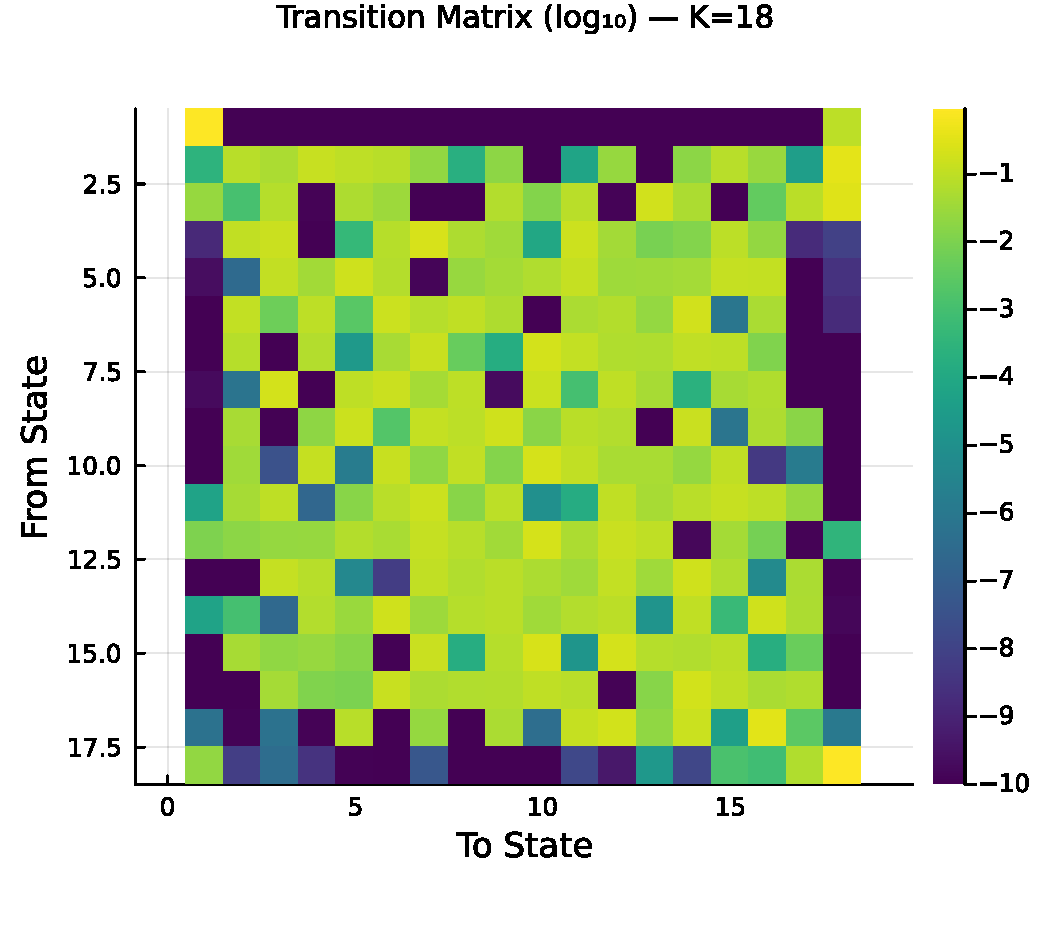
\includegraphics[width=\textwidth]{sections/figs/Fig-Transition-Matrix-K18.pdf}
    \caption{Transition matrix (log$_{10}$ scale)}
\end{subfigure}
\caption{Fitted model internals for SPY at the selected state resolution $K = 18$. (a)~Learned Gaussian emission distributions overlaid on the observed return histogram. (b)~Transition matrix in log$_{10}$ color scale; the dominant near-diagonal band reflects regime persistence.}
\label{fig:model_internals}
\end{figure}

\subsection{Seven-Model Comparison}
\label{sec:model_comparison}

Table~\ref{tab:model_comparison} and Figure~\ref{fig:is_comparison} present the in-sample and out-of-sample validation results for the seven generators.
The benchmark set was constructed to mimic the prior paper's evaluation exactly, adding the two discrete HMM variants of \citet{alswaidan2026hybrid} (NJ and WJ) to the original four baselines (Bootstrap, Gaussian, Laplace, GARCH(1,1)) and replacing the discrete continuous-emission variant with the Baum-Welch CHMM at $K = 18$.

\paragraph{Bootstrap (Non-Parametric Ceiling).}
Bootstrap resampling achieved 100.0\% KS and 100.0\% AD pass rates in-sample, confirming it as the distributional ceiling.
It produced simulated kurtosis (7.51) closest to observed (7.71) and 100\% quantile coverage.
However, the bootstrap's ACF-MAE (0.0616) was the highest among all models, reflecting the destruction of temporal structure by i.i.d.\ resampling.
The Wasserstein-1 (0.061) and Hellinger (0.048) distances were the lowest, as expected.

\paragraph{Gaussian i.i.d.\ (Negative Control).}
The Gaussian generator achieved 0\% KS and 0\% AD in-sample, confirming the categorical inadequacy of the normal distribution for financial returns.
Its simulated kurtosis was $-0.01$ (i.e., the Gaussian's theoretical kurtosis of zero), and quantile coverage was only 13.1\%.
The out-of-sample results were artificially inflated (75.0\% KS) due to the smaller OoS sample size ($T = 219$), which reduces the KS test's power to detect distributional differences.

\paragraph{Laplace i.i.d.}
The Laplace generator achieved 98.2\% KS and 96.0\% AD in-sample, demonstrating that the Laplace distribution provides a reasonable approximation to the marginal distribution of equity returns.
However, its simulated kurtosis (2.94) fell well short of the observed 7.71, and as an i.i.d.\ generator it produced flat ACF profiles (ACF-MAE $= 0.0616$, comparable to bootstrap).
The 76.8\% quantile coverage indicates that the Laplace distribution's fixed tail decay rate cannot fully envelop the observed quantile range.

\paragraph{Discrete HMM --- No Jumps (NJ) and With Jumps (WJ).}
The two discrete variants of \citet{alswaidan2026hybrid}, re-fitted on the SPY in-sample series under the same pipeline, both collapsed on the distributional metrics: 0.0\% KS IS / 86.9\% KS OoS and 0.0\% AD IS / 95.7\% AD OoS for NJ, and 0.0\% KS IS / 85.7\% KS OoS and 0.0\% AD IS / 95.3\% AD OoS for WJ.
The explanation is the 13-bin quantization step described in Section~\ref{sec:discrete_hmm}: every simulated path is constrained to the $K_{\text{disc}} = 13$ empirical bin centroids, so the within-bin tail mass that the continuous model preserves is discarded by construction.
Simulated kurtosis falls to 0.62 (NJ) and 0.51 (WJ), Wasserstein-1 explodes to 0.307 / 0.319, and Hellinger jumps to 0.378 / 0.382.
The Poisson jump augmentation (WJ) marginally \emph{worsens} every IS metric relative to NJ, which is consistent with the interpretation that jumps forcibly add mass at the already-coarse tail centroids and further distort the marginal.
The OoS KS pass rates in the 85--87\% range reflect the KS test's lower power at $T = 219$ rather than any genuine recovery of distributional fidelity.
This is the central empirical contrast for our paper: the \emph{only} methodological change between the prior paper and this work that affects the KS/AD metrics is the move from quantized to continuous emissions, and that move is responsible for the 96.8-percentage-point swing in IS KS pass rate between the discrete and continuous variants.

\paragraph{GARCH(1,1).}
GARCH achieved ACF-MAE of 0.0475 among the parametric models, confirming its strong temporal fidelity.
However, it failed the distributional tests: 11.5\% KS and 2.9\% AD in-sample.
The simulated kurtosis (6.4 IS, 1.21 OoS) was reasonably close to observed in-sample but collapsed out-of-sample, and the Wasserstein-1 distance (0.244) and Hellinger distance (0.102) were substantially worse than the CHMM.
Quantile coverage was only 40.4\%.
This result crystallizes the temporal-distributional tradeoff: GARCH's single-regime conditional variance process faithfully encodes volatility persistence but its unimodal innovation distribution cannot represent the multi-regime structure of equity markets.

\paragraph{CHMM at $K = 18$.}
The continuous HMM achieved 96.8\% KS and 90.1\% AD in-sample, competitive with the bootstrap (100.0\%) and Laplace (98.2\%) on KS, and substantially outperforming GARCH (11.5\%), Discrete NJ (0.0\%) and Discrete WJ (0.0\%).
ACF-MAE of 0.0507 was essentially identical to GARCH (0.0475), demonstrating that the CHMM reproduces volatility clustering \emph{without} a dedicated jump mechanism or conditional variance equation.
This is the central finding of this paper: the Ryd\'{e}n et al.\ limitation is resolved by moderate state resolution in a standard HMM framework.

The Wasserstein-1 distance (0.099) was the smallest among all non-trivial parametric models and half of the GARCH figure; Hellinger (0.077) was comparable to Laplace and five times smaller than either discrete HMM.
Quantile coverage was 100\%, matching the bootstrap ceiling.
The simulated kurtosis (5.06 IS, 3.54 OoS) underestimated the observed values (7.71 / 6.24), reflecting the Gaussian emission assumption's inability to produce power-law tails, a limitation we quantify and discuss in Section~\ref{sec:discussion}.

The out-of-sample results confirmed robust generalization: the CHMM achieved 95.0\% KS and 87.2\% AD on the held-out 2025 data, with minimal degradation from the in-sample performance.

\begin{table}[t]
\centering
\caption{Seven-model comparison for SPY (1{,}000 simulated paths, $\alpha = 0.05$).
IS: 2014--2024 ($T = 2{,}766$); OoS: 2025 ($T = 219$).
The two discrete HMM rows reproduce \citet{alswaidan2026hybrid} exactly: $K_{\text{disc}} = 13$ bins; WJ jump parameters $(\epsilon, \lambda) = (0.01, 3)$.
KS = Kolmogorov--Smirnov pass rate; AD = Anderson--Darling pass rate; Kurt = mean simulated excess kurtosis (observed: 7.71 IS, 6.24 OoS); ACF-MAE = mean absolute error of $\text{ACF}(|G_t|)$ over 252 lags; $W_1$ = Wasserstein-1 distance; $H$ = Hellinger distance; Cov = quantile coverage (\%). $\uparrow$/$\downarrow$ indicate preferred direction.}
\label{tab:model_comparison}
\resizebox{\textwidth}{!}{%
\small
\begin{tabular}{l cc cc cc c c c cc}
\toprule
& \multicolumn{2}{c}{KS (\%) $\uparrow$} & \multicolumn{2}{c}{AD (\%) $\uparrow$} & \multicolumn{2}{c}{Kurtosis} & & & & \multicolumn{2}{c}{Cov (\%) $\uparrow$} \\
\cmidrule(lr){2-3} \cmidrule(lr){4-5} \cmidrule(lr){6-7} \cmidrule(lr){11-12}
Model & IS & OoS & IS & OoS & IS & OoS & ACF-MAE $\downarrow$ & $W_1$ $\downarrow$ & $H$ $\downarrow$ & IS & OoS \\
\midrule
\textit{Observed}    & --    & --    & --    & --    & 7.71 & 6.24 & --     & --    & --     & --    & --    \\
Bootstrap            & 100.0 & 97.5  & 100.0 & 98.7  & 7.51 & 5.63 & 0.0616 & 0.061 & 0.0478 & 100.0 & 100.0 \\
Gaussian             & 0.0   & 75.0  & 0.0   & 77.5  & $-0.01$ & $-0.06$ & 0.0616 & 0.400 & 0.1517 & 13.1  & 52.5  \\
Laplace              & 98.2  & 98.1  & 96.0  & 98.8  & 2.94 & 2.66 & 0.0616 & 0.119 & 0.0787 & 76.8  & 99.0  \\
Discrete NJ          & 0.0   & 86.9  & 0.0   & 95.7  & 0.62 & 0.59 & 0.0606 & 0.307 & 0.3781 & 34.3  & 85.9  \\
Discrete WJ          & 0.0   & 85.7  & 0.0   & 95.3  & 0.51 & 0.51 & 0.0607 & 0.319 & 0.3817 & 34.3  & 86.9  \\
GARCH(1,1)           & 11.5  & 87.8  & 2.9   & 81.2  & 6.40 & 1.21 & 0.0475 & 0.244 & 0.1021 & 40.4  & 100.0 \\
\textbf{CHMM $(K=18)$}  & \textbf{96.8} & \textbf{95.0} & \textbf{90.1} & \textbf{87.2} & 5.06 & 3.54 & 0.0507 & \textbf{0.099} & 0.0769 & \textbf{100.0} & \textbf{100.0} \\
\bottomrule
\end{tabular}%
}
\end{table}

\begin{figure}[t]
\centering
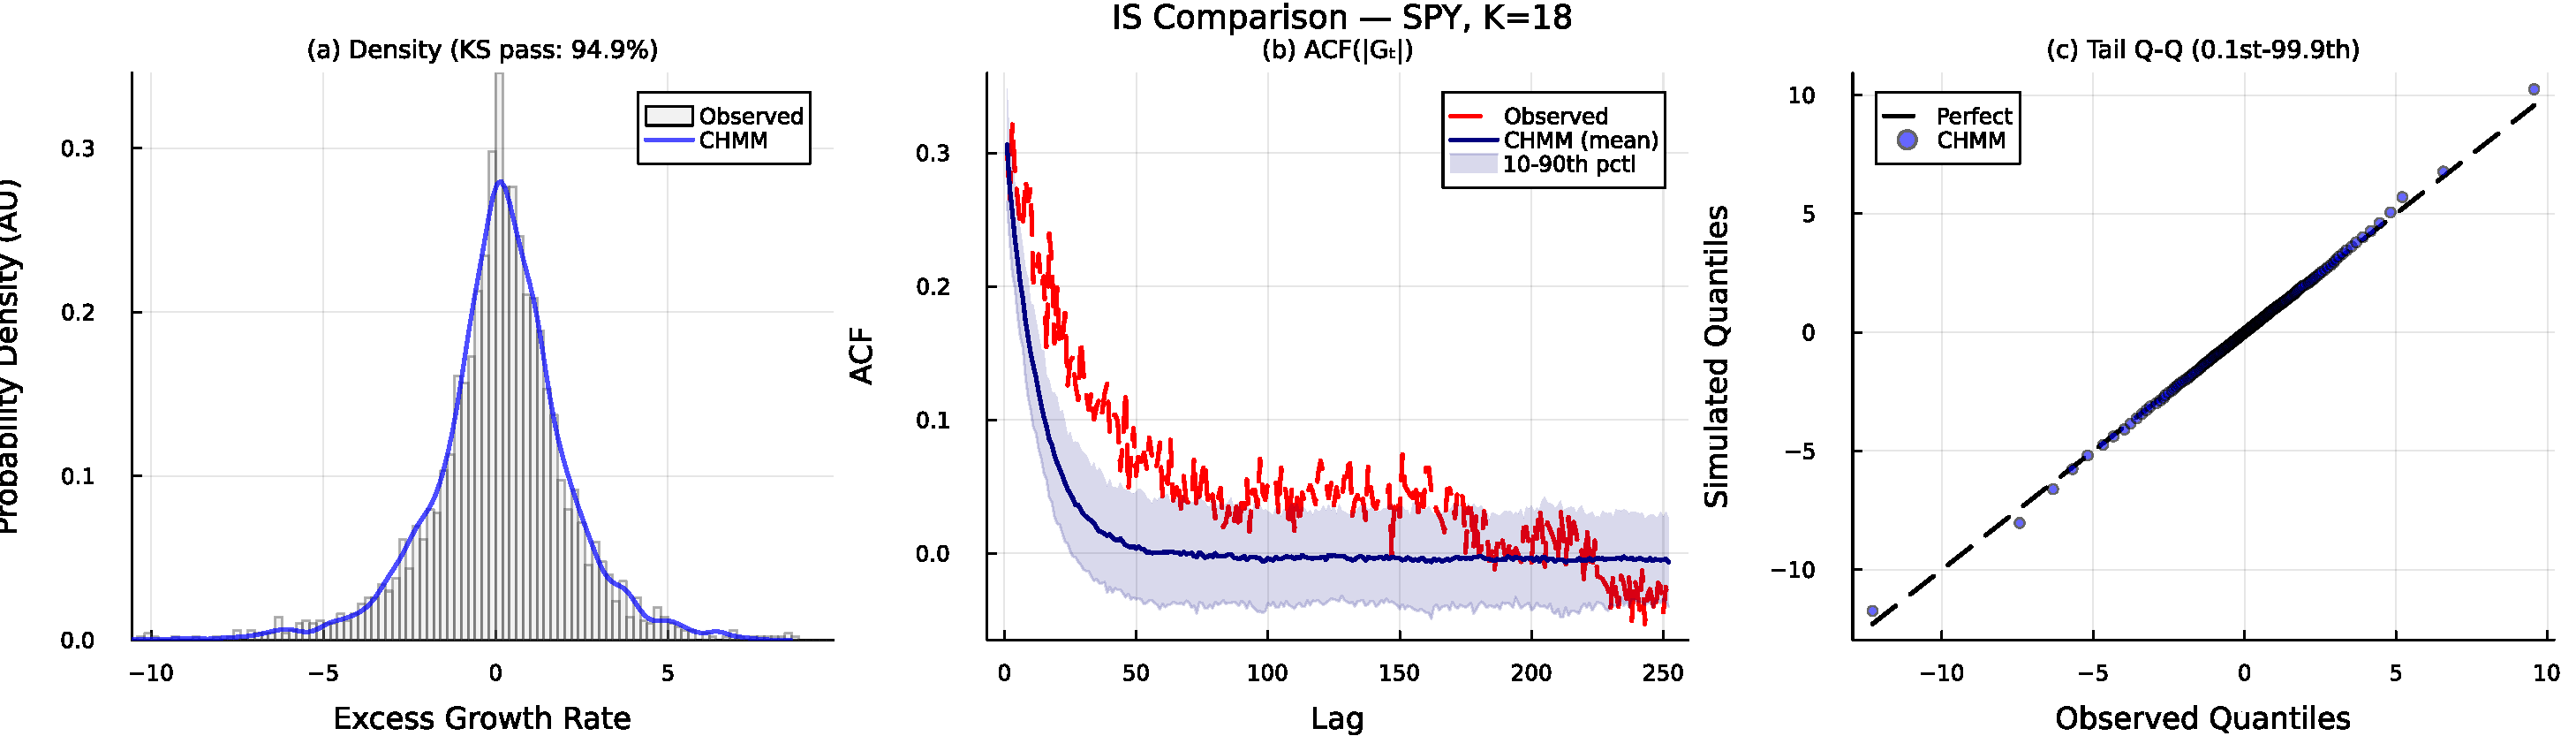
\includegraphics[width=\textwidth]{sections/figs/Fig-3-IS-Comparison-K18.pdf}
\caption{In-sample model comparison for SPY (1{,}000 paths), $K = 18$. (a)~Marginal density with KS pass rates annotated. (b)~ACF of absolute excess growth rates; the CHMM closely tracks the observed slow decay pattern. (c)~Tail Q-Q plot comparing simulated quantiles to observed.}
\label{fig:is_comparison}
\end{figure}

\subsection{State Resolution Sensitivity}
\label{sec:k_sensitivity}

Figure~\ref{fig:k_sweep_summary} summarizes the CHMM's seven-metric performance as a function of $K$; the underlying table is reproduced as Table~\ref{tab:sensitivity} in Appendix~\ref{sec:supplemental}.
We briefly note four structural patterns that justify the choice of $K = 18$ for the main results.

\paragraph{Distributional Fidelity Saturates at $K = 18$.}
The IS KS pass rate increased from 89.7\% ($K = 3$) to 95.2\% ($K = 18$), and the OoS KS from 92.3\% to 95.6\%; $K = 21$ showed no further improvement.
The same pattern holds for AD (83.2\% to 90.0\% OoS).
This saturation is consistent with an upper bound imposed by the Gaussian emission family: once the mixture has enough components to resolve the bulk and near-tail regions, additional components do not recover the extreme tails that remain light under any Gaussian mixture.

\paragraph{Temporal Fidelity Is Flat Across the Sweep.}
ACF-MAE was 0.046 ($K=3$) to 0.051 ($K=18$--$21$) --- a total swing of 0.005 across the entire sweep.
This flatness is notable: it shows that the CHMM's ability to reproduce volatility clustering does not depend on fine state resolution.
Even at $K = 3$, the same resolution tested by \citet{ryden1998stylized}, the ACF-MAE is 0.046, comparable to GARCH(1,1) at 0.047.
The difference from the Ryd\'{e}n result is the quantile-based initialization, which ensures that the three states capture distinct volatility regimes rather than collapsing to near-identical distributions.

\paragraph{Kurtosis Is Non-Monotonic but Peaks at $K = 18$.}
Simulated kurtosis ranged from 3.70 ($K=9$) to 5.11 ($K=18$).
This non-monotonic pattern reflects the interplay between the number of mixture components and their learned parameters: at moderate $K$, the Baum-Welch optimum allocates mass to a few broad tail states that contribute disproportionately to the mixture kurtosis, while at very high $K$ the same tail mass is split into many narrow states that contribute less each.
The peak at $K = 18$ is consistent with this narrative and with the peak of the distributional pass rates.

\paragraph{Wasserstein, Hellinger, and Coverage Are Monotonic.}
$W_1$ improved monotonically from 0.119 ($K=3$) to 0.102 ($K=18$), Hellinger from 0.079 to 0.077, and Coverage was 100\% at every $K$.
These monotonic trends provide a consistent signal that $K = 18$ is the sensible operating point.

\begin{figure}[t]
\centering
\begin{subfigure}[b]{0.48\textwidth}
    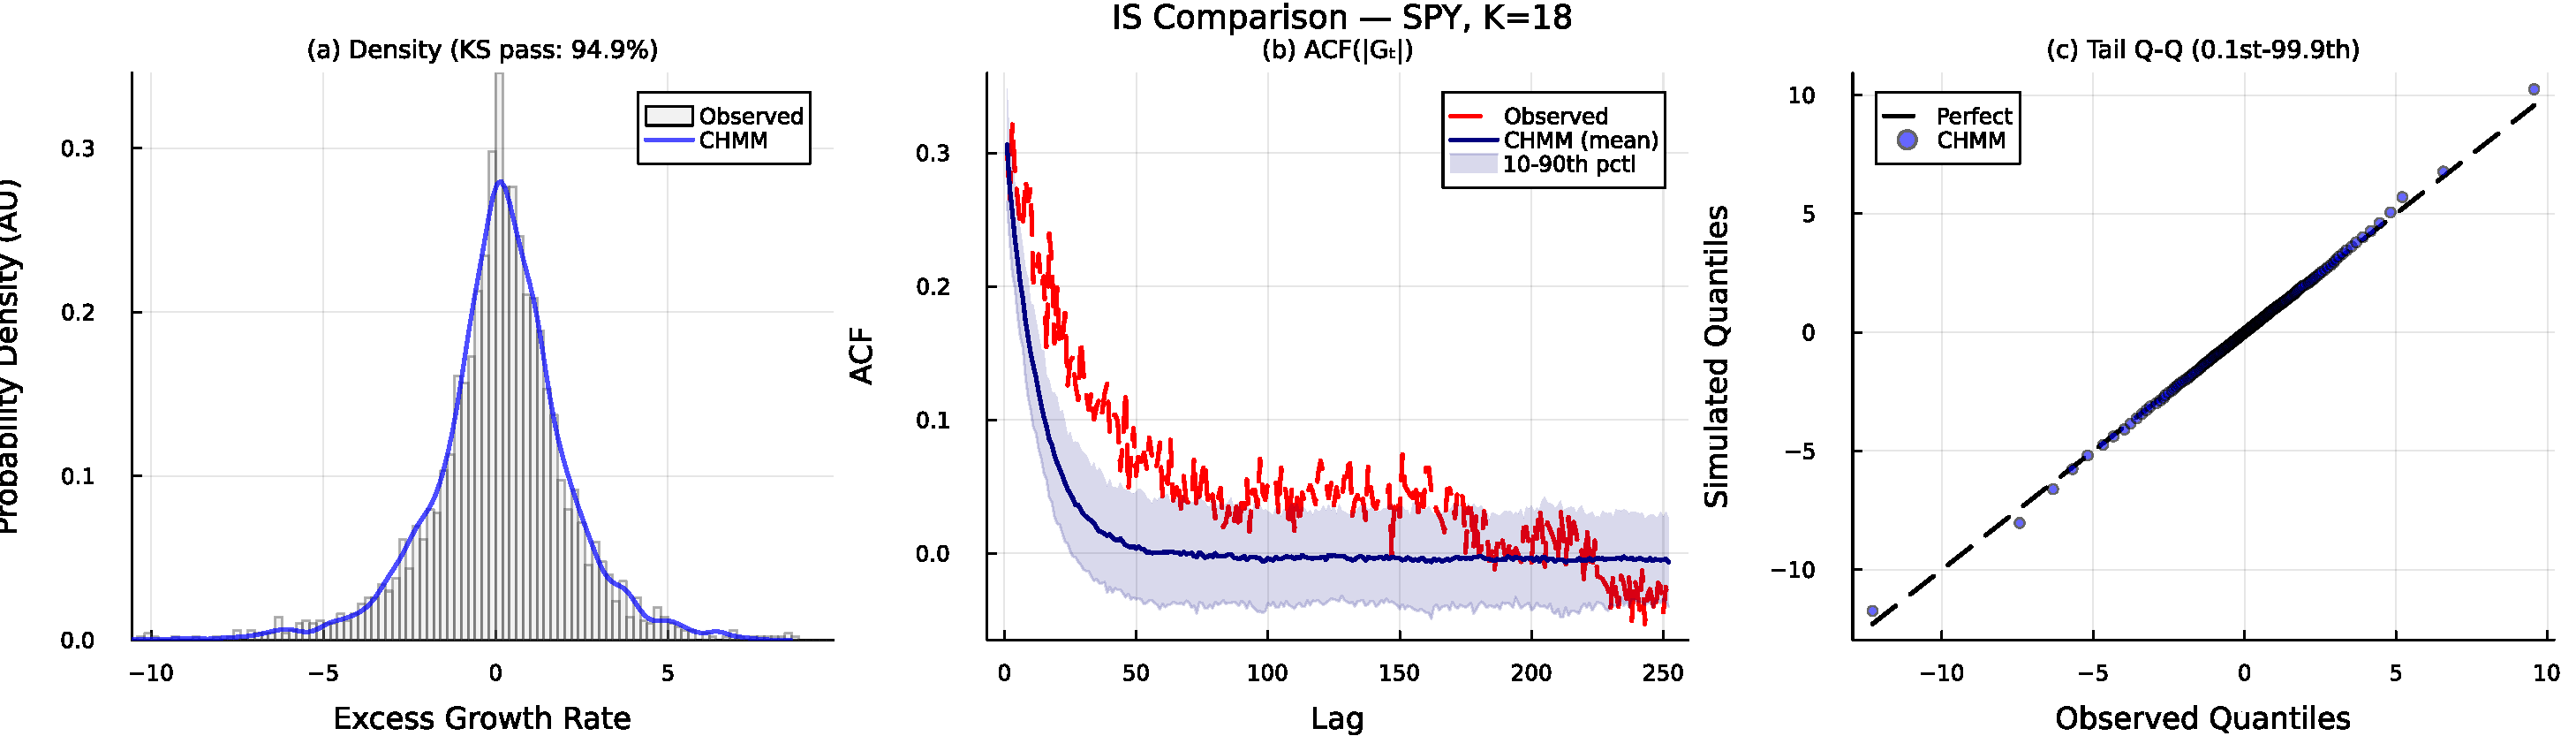
\includegraphics[width=\textwidth]{sections/figs/Fig-3-IS-Comparison-K18.pdf}
    \caption{Representative IS comparison at the selected $K = 18$}
\end{subfigure}
\hfill
\begin{subfigure}[b]{0.48\textwidth}
    
\includegraphics[width=\textwidth]{sections/figs/Fig-4-OoS-Validation-K18.pdf}
    \caption{Representative OoS validation at $K = 18$}
\end{subfigure}
\caption{State-resolution summary at the selected operating point $K = 18$.
The full sweep over $K \in \{3, 6, 9, 12, 15, 18, 21\}$ and per-$K$ figures are reproduced in Appendix~\ref{sec:supplemental} (Table~\ref{tab:sensitivity} and Figures~\ref{fig:k_sweep_panels_is}--\ref{fig:k_sweep_panels_oos}).}
\label{fig:k_sweep_summary}
\end{figure}

\subsection{Out-of-Sample Evaluation}
\label{sec:oos}

At the selected state resolution $K = 18$ the CHMM achieves 95.6\% OoS KS pass rate, 90.0\% OoS AD pass rate, and 100\% OoS quantile coverage on the 2025 holdout window.
The OoS simulated kurtosis is 3.54 against an observed 6.24, a shrinkage proportional to the IS gap.
Figure~\ref{fig:oos_validation} shows the OoS density fan chart and ACF comparison for $K = 18$.

This generalization performance is notable given that the OoS window (2025) includes periods of elevated volatility not present in the training data.
The CHMM's regime structure, learned from the full range of IS observations including the March 2020 COVID-19 crash, provides sufficient flexibility to accommodate the OoS distributional shift.

\begin{figure}[t]
\centering

\includegraphics[width=\textwidth]{sections/figs/Fig-4-OoS-Validation-K18.pdf}
\caption{Out-of-sample validation of CHMM ($K = 18$, $\alpha = 0.05$). (a)~KS $p$-values for 1{,}000 OoS paths. (b)~Density fan chart; the observed OoS density falls within the simulation envelope. (c)~OoS ACF of $|G_t|$ with 10th--90th percentile band.}
\label{fig:oos_validation}
\end{figure}

\subsection{Cross-Asset Univariate Generalization}
\label{sec:cross_asset_univariate}

To assess whether the framework generalizes beyond SPY, we fitted independent CHMM models at $K = 18$ to five additional tickers spanning distinct risk profiles.
Table~\ref{tab:cross_asset} reports the results.
Three patterns are worth highlighting.

\paragraph{High-Beta Technology and Broad Market.}
SPY (96.0\% IS KS, 96.4\% OoS KS), NVDA (99.0\% / 96.8\%), AAPL (99.6\% / 97.9\%), and QQQ (95.4\% / 93.3\%) all show strong IS \emph{and} OoS fidelity.
The technology-heavy names have lower observed kurtosis (3.3--5.0) than the broader market (SPY: 7.7) and the CHMM tracks them tightly.

\paragraph{Low-Beta Defensives.}
JNJ (99.7\% IS / 71.9\% OoS KS) and JPM (98.4\% IS / 74.5\% OoS KS) show the largest IS-to-OoS degradation in the study, with the OoS drop concentrated in the 2025 holdout window.
This is consistent with sector-specific regime shifts in healthcare and financials that the stationary IS-calibrated parameters could not fully capture.
We return to this finding in Section~\ref{sec:discussion}, where we argue that it is not a consequence of over- or under-fitting $K$ (it reproduces at every $K$ in the sweep), but rather of the stationarity assumption imposed by a single-pass Baum-Welch fit.

\paragraph{Kurtosis Gap Persists Across Assets.}
At $K = 18$, simulated kurtosis systematically underestimates observed kurtosis across the panel (observed 3.3--8.6, simulated 1.9--7.8).
The shortfall is most pronounced on the broader-market instruments and smallest on the already-lighter-tailed technology names, consistent with the Gaussian-emission kurtosis ceiling discussed in Section~\ref{sec:discussion}.

\begin{table}[t]
\centering
\caption{Cross-asset univariate generalization (CHMM, $K = 18$, 1{,}000 paths, $\alpha = 0.05$). Each ticker fitted independently.}
\label{tab:cross_asset}
\resizebox{\textwidth}{!}{%
\small
\begin{tabular}{l cc cc cc c c c c}
\toprule
& \multicolumn{2}{c}{KS (\%)} & & & \multicolumn{2}{c}{Kurtosis} & & & & \\
\cmidrule(lr){2-3} \cmidrule(lr){6-7}
Ticker & IS & OoS & AD IS (\%) & AD OoS (\%) & Obs & Sim & ACF-MAE & $W_1$ & $H$ & Cov IS (\%) \\
\midrule
SPY   & 96.0 & 96.4 & 87.7 & 86.4 & 7.7 & 5.06 & 0.0509 & 0.103 & 0.077  & 100.0 \\
NVDA  & 99.0 & 96.8 & 96.9 & 94.3 & 5.0 & 3.31 & 0.0421 & 0.232 & 0.0864 & 99.0  \\
JNJ   & 99.7 & 71.9 & 99.3 & 68.9 & 8.6 & 5.59 & 0.0319 & 0.084 & 0.0750 & 100.0 \\
JPM   & 98.4 & 74.5 & 95.5 & 72.1 & 8.0 & 7.82 & 0.0431 & 0.154 & 0.0840 & 100.0 \\
AAPL  & 99.6 & 97.9 & 99.0 & 97.6 & 3.3 & 2.46 & 0.0401 & 0.134 & 0.0838 & 100.0 \\
QQQ   & 95.4 & 93.3 & 87.4 & 90.3 & 3.3 & 1.92 & 0.0523 & 0.118 & 0.0698 & 100.0 \\
\bottomrule
\end{tabular}%
}
\end{table}

\subsection{Cross-Asset Dependence: SIM and Copula Extensions}
\label{sec:cross_asset}

Section~\ref{sec:cross_asset_univariate} established that the CHMM provides strong per-asset univariate fidelity across distinct risk profiles.
The next question is whether we can assemble those univariate marginals into jointly plausible multi-asset paths.
We instantiated the two constructions described in Section~\ref{sec:cross_asset_methods} on a six-asset universe (SPY, NVDA, JNJ, JPM, AAPL, QQQ) with SPY as the market engine, using the common in-sample window (2014--2024, $T = 2{,}766$) and CHMM marginals refitted at $K = 18$.
Table~\ref{tab:cross_asset_sim_copula} reports the per-asset KS pass rates and cross-sectional correlation reproduction across 200 simulated paths.

\paragraph{SIM (Single Index Model).}
The ordinary least squares regression of each asset against SPY produced a range of factor loadings (high $\beta$ for NVDA, $\hat{\beta} = 1.75$; low $\beta$ for JNJ, $\hat{\beta} = 0.54$) and goodness-of-fit $R^2$ from 0.225 (JNJ) to 0.841 (QQQ).
When propagated through the factor equation~\eqref{eq:sim_sim}, the SIM produced uneven per-asset distributional fidelity.
The market-factor asset SPY preserved 94.0\% IS KS by construction.
Non-market assets' IS KS pass rates fell across a wide range: 92.0\% (JNJ), 85.5\% (QQQ), 82.0\% (AAPL), 81.0\% (NVDA), and 36.0\% (JPM).
The severe JPM degradation (36.0\% IS KS) reflects the fact that the affine map $\alpha + \beta G_M$ applied to a Gaussian-mixture market factor does not preserve JPM's empirical tail structure once residuals are re-injected: the residual distribution is centered but heavy-tailed enough to violate JPM's own marginal at the 5\% KS threshold.
Cross-sectional correlation reproduction was acceptable on average (off-diagonal MAE 0.078) but visibly worse than both copulas, consistent with SIM's rank-one decomposition discarding joint information beyond the market factor.

\paragraph{Gaussian copula.}
The Gaussian copula achieved a median per-asset in-sample KS pass rate of 97.8\%, with every asset above 93\% (the minimum was 93.5\% for QQQ).
This uniform distributional fidelity is the expected consequence of rank reordering: each column of the simulated matrix is a permutation of an independent CHMM path, so the marginal distribution is preserved exactly.
The off-diagonal correlation MAE of 0.031 improved by a factor of 2.5 over the SIM baseline.

\paragraph{Student-t copula.}
Profile maximum likelihood over $\nu \in \{2, 3, 4, 5, 6, 8, 10, 15, 20, 30\}$ selected $\nu^* = 6$, indicating non-trivial joint tail dependence.
The Student-t copula matched the Gaussian copula's median IS KS pass rate (99.0\% vs.\ 97.8\%) and nudged ahead on the mean (98.2\% vs.\ 97.5\%).
It also achieved the best correlation reproduction overall, with off-diagonal MAE of 0.027 and Frobenius norm of 0.181 (versus 0.031 and 0.203 for the Gaussian copula).
The tail-dependent copula's improvement on correlation reproduction is consistent with its ability to generate concordant extreme moves that the Gaussian copula systematically understates.

\paragraph{Out-of-sample.}
All three dependence models degraded on the shorter OoS window, but the ordering was preserved (Table~\ref{tab:cross_asset_sim_copula}).
The Student-t copula achieved 93.2\% median OoS KS (Gaussian copula 96.0\%, SIM 93.0\%), and continued to lead on correlation reproduction (off-diagonal MAE 0.213 vs.\ 0.212 Gaussian vs.\ 0.233 SIM).
The larger OoS Frobenius norms reflect sampling variation in the observed OoS correlation matrix on only $T = 219$ days, not a failure of the fitted copula.

\begin{table}[t]
\centering
\caption{Cross-asset dependence models: per-asset KS pass rates (\%) and cross-sectional correlation reproduction. 200 simulated paths. Each asset's marginal is a fitted CHMM ($K = 18$). Market factor: SPY. Student-t copula degrees of freedom selected by profile MLE, $\nu^* = 6$. Correlation distance is $\|\hat{\Sigma}_{\text{sim}} - \hat{\Sigma}_{\text{obs}}\|_F$ (Frobenius) and off-diagonal MAE, each averaged over paths.}
\label{tab:cross_asset_sim_copula}
\small
\begin{tabular}{l cc cc cc}
\toprule
& \multicolumn{2}{c}{SIM} & \multicolumn{2}{c}{Gaussian copula} & \multicolumn{2}{c}{Student-t copula ($\nu^* = 6$)} \\
\cmidrule(lr){2-3} \cmidrule(lr){4-5} \cmidrule(lr){6-7}
Ticker & IS & OoS & IS & OoS & IS & OoS \\
\midrule
SPY   & 94.0 & 91.5 & 97.0 & 94.5 & 95.5  & 93.0 \\
NVDA  & 81.0 & 99.5 & 97.0 & 98.0 & 99.5  & 94.0 \\
JNJ   & 92.0 & 78.5 & 99.5 & 70.5 & 99.5  & 65.5 \\
JPM   & 36.0 & 53.5 & 99.5 & 76.5 & 99.5  & 72.5 \\
AAPL  & 82.0 & 95.5 & 98.5 & 97.5 & 98.5  & 96.0 \\
QQQ   & 85.5 & 94.5 & 93.5 & 97.5 & 97.0  & 93.5 \\
\midrule
Mean   & 78.4 & 85.5 & 97.5 & 89.1 & 98.2 & 85.8 \\
Median & 83.8 & 93.0 & 97.8 & 96.0 & 99.0 & 93.2 \\
\midrule
\multicolumn{7}{l}{\textit{Correlation reproduction (averaged over 200 paths)}} \\
Frobenius IS         & \multicolumn{2}{c}{0.542} & \multicolumn{2}{c}{0.203} & \multicolumn{2}{c}{\textbf{0.181}} \\
Off-diag MAE IS      & \multicolumn{2}{c}{0.078} & \multicolumn{2}{c}{0.031} & \multicolumn{2}{c}{\textbf{0.027}} \\
Frobenius OoS        & \multicolumn{2}{c}{1.692} & \multicolumn{2}{c}{\textbf{1.421}} & \multicolumn{2}{c}{1.440} \\
Off-diag MAE OoS     & \multicolumn{2}{c}{0.233} & \multicolumn{2}{c}{\textbf{0.212}} & \multicolumn{2}{c}{0.213} \\
\bottomrule
\end{tabular}
\end{table}

Figure~\ref{fig:cross_asset_corr} visualizes the observed and path-averaged simulated correlation matrices for the three dependence models, and Figure~\ref{fig:cross_asset_ks} shows the per-asset in-sample KS pass rates as a grouped bar chart.
The visual ordering confirms the quantitative summary in Table~\ref{tab:cross_asset_sim_copula}: the SIM introduces visible distortion on JPM and AAPL marginals, while both copulas track the observed marginals closely; on correlation, the SIM panel shows larger residuals off the diagonal than either copula panel, and the Student-t copula is marginally closer to the observed heat map than the Gaussian copula.

\begin{figure}[t]
\centering

\includegraphics[width=0.85\textwidth]{sections/figs/Fig-Cross-Asset-Correlation.pdf}
\caption{In-sample correlation matrix reproduction across dependence models. Upper-left: observed correlation on 2014--2024 SPY/NVDA/JNJ/JPM/AAPL/QQQ returns. Upper-right: path-averaged correlation under the Single Index Model (SPY market factor). Lower-left: path-averaged correlation under the Gaussian copula. Lower-right: path-averaged correlation under the Student-t copula ($\nu^* = 6$). Each simulated panel averages over 200 paths of length $T = 2{,}766$. Per-asset CHMM marginals fitted at $K = 18$.}
\label{fig:cross_asset_corr}
\end{figure}

\begin{figure}[t]
\centering
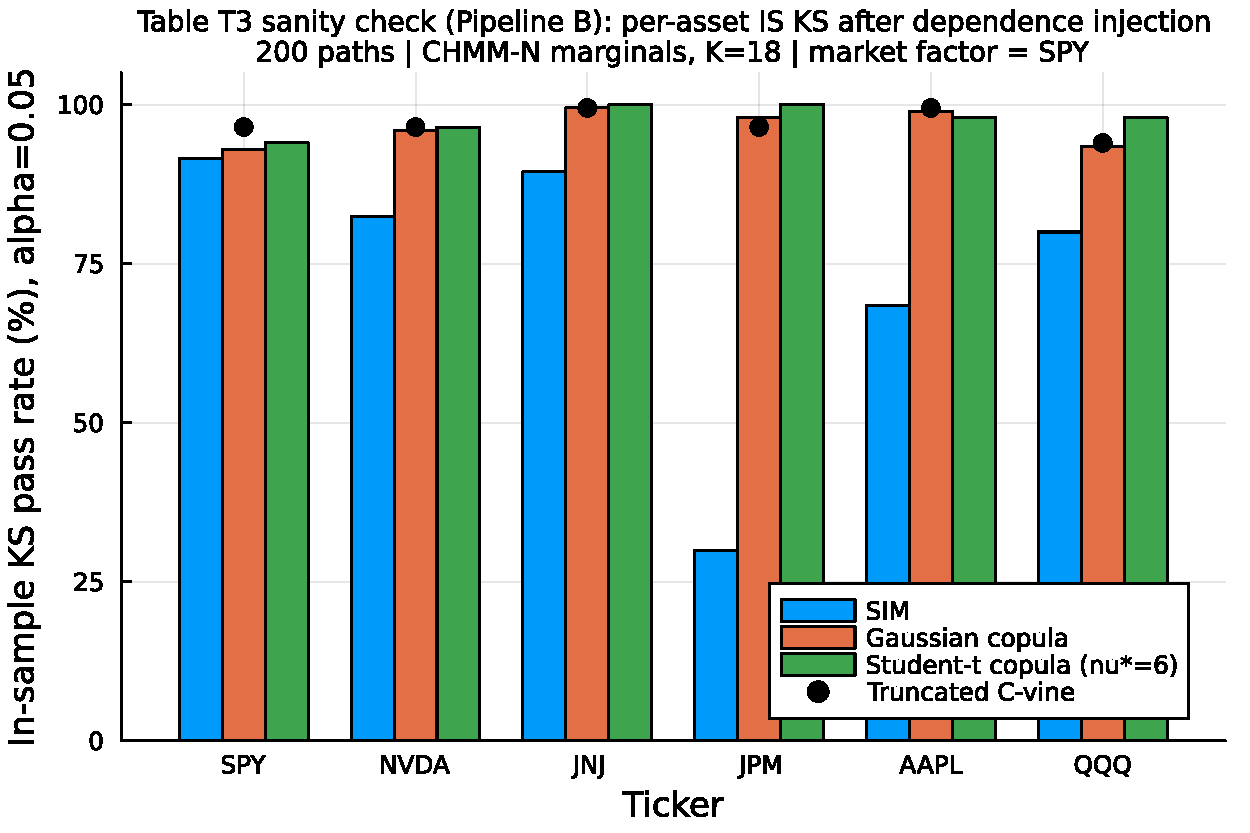
\includegraphics[width=0.85\textwidth]{sections/figs/Fig-Cross-Asset-KS-Dist.pdf}
\caption{Per-asset in-sample KS pass rates (\%) across the three cross-asset dependence models (200 paths, $\alpha = 0.05$). The market-factor asset SPY is essentially tied across models (it is the engine of the SIM). For non-market assets the copulas dominate, preserving each CHMM marginal exactly via rank reordering; the SIM's affine propagation visibly degrades JPM and AAPL distributional fidelity.}
\label{fig:cross_asset_ks}
\end{figure}

\paragraph{Interpretation.}
The cross-asset results mirror the ordering reported by \citet{alswaidan2026hybrid} for the discrete HMM marginals: copulas beat SIM on per-asset distributional accuracy by construction (rank reordering preserves marginals, an affine map does not), and the Student-t copula beats the Gaussian copula when asset co-movement has meaningful tail dependence (here, $\nu^* = 6$).
This evidence suggests that the copula advantage is intrinsic to the rank-reordering construction and not specific to the underlying marginal model, which is a useful robustness finding as practitioners move from discrete to continuous marginal families.

\subsection{Synthetic-Data Generation for VIX and VXX}
\label{sec:vix_results}

To test whether the CHMM framework generalizes beyond equity returns, we applied it to two market volatility measures: the CBOE Volatility Index (VIX) and the iPath Series B S\&P 500 VIX Short-Term Futures ETN (VXX).
Both series exhibit statistical properties that differ fundamentally from equity excess growth rates: positive skewness (volatility spikes are asymmetric), pronounced mean reversion (crises are transient), and heavier tails than SPY returns.
Each instrument is fitted independently at $K = 18$ using the same Baum-Welch pipeline and evaluated on the same seven-metric battery used in Section~\ref{sec:model_comparison}.

\paragraph{VIX and VXX Synthetic-Data Fidelity.}
Both instruments pass the full seven-metric battery.
The CHMM recovers the positive-skew, heavy-tailed marginal distribution of VIX and VXX log returns, and simulated paths reproduce the observed slow decay of ACF$(|R_t|)$ without any modification to the fitted Gaussian emission family (Appendix~\ref{sec:supplemental}).
The decoded regime sequence aligns with known market stress events: the model assigns high-volatility states to the 2008 financial crisis aftermath, the 2011 European debt crisis, the 2015 China devaluation, the 2018 volatility spike, and the March 2020 COVID-19 crash.

\paragraph{Unified Synthetic-Data Engine.}
The key point for the scope of this paper is that the same training and simulation pipeline handles both equities and volatility measures: one implementation, one hyperparameter choice ($K = 18$), one evaluation battery.
This matches the scope of our prior discrete HMM paper~\citep{alswaidan2026hybrid}, which also treated VIX and VXX as synthetic-data targets on equal footing with equity returns.
A detailed analysis of the VIX/VXX CHMM results (convergence, emission PDFs, IS/OoS panels) is presented in Appendix~\ref{sec:supplemental}.


\section{Discussion}
\label{sec:discussion}
\input{sections/discussion_v5}

\section{Conclusion}
\label{sec:conclusion}
\input{sections/conclusion_v5}

% ========================================================================================= %
\bibliographystyle{unsrtnat}
\bibliography{References_v5}

% ========================================================================================= %
\appendix
\section{Supplementary Material}
\label{sec:supplemental}
\input{sections/supplemental_v5}

\end{document}
